\begin{enumerate}[label=\thechapter.\arabic*,ref=\thechapter.\theenumi]
\item The causal signal with Z transform $z^2(z - a)^{-2}$ is ($u(n)$ is unit step signal)
\begin{enumerate}
    \item $a^{2n}u(n)$
    \item $(n + 1)a^nu(n)$
    \item $n^{-1}a^nu(n)$
    \item $n^2a^nu(n)$
\end{enumerate}

\hfill(GATE 31 EE 2021) 

\solution
 \iffalse
\let\negmedspace\undefined
\let\negthickspace\undefined
\documentclass[journal,12pt,twocolumn]{IEEEtran}
\usepackage{cite}
\usepackage{amsmath,amssymb,amsfonts,amsthm}
\usepackage{algorithmic}
\usepackage{graphicx}
\usepackage{textcomp}
\usepackage{xcolor}
\usepackage{txfonts}
\usepackage{listings}
\usepackage{enumitem}
\usepackage{mathtools}
\usepackage{gensymb}
\usepackage{comment}
\usepackage[breaklinks=true]{hyperref}
\usepackage{tkz-euclide} 
\usepackage{tikz}
% \usetikzlibrary{positioning, arrows.meta}
\usepackage{listings}
\usepackage{gvv} 
\usepackage{caption}
\def\inputGnumericTable{}                   

%\usepackage[latin1]{inputenc}                                
\usepackage{color}                                            
\usepackage{array}                                            
\usepackage{longtable}                                       
\usepackage{calc}                                             
\usepackage{multirow}                                         
\usepackage{hhline}                                           
\usepackage{ifthen}                                           
\usepackage{lscape}
\usepackage{tikz}
\newtheorem{theorem}{Theorem}[section]
\newtheorem{problem}{Problem}
\newtheorem{proposition}{Proposition}[section]
\newtheorem{lemma}{Lemma}[section]
\newtheorem{corollary}[theorem]{Corollary}
\newtheorem{example}{Example}[section]
\newtheorem{definition}[problem]{Definition}
\newcommand{\BEQA}{\begin{eqnarray}}
\newcommand{\EEQA}{\end{eqnarray}}
\newcommand{\define}{\stackrel{\triangle}{=}}
\theoremstyle{remark}
\newtheorem{rem}{Remark}

\begin{document}

\bibliographystyle{IEEEtran}
\vspace{3cm}

\title{GATE: EE - 31.2021}
\author{EE23BTECH11013 - Avyaaz$^{*}$% <-this % stops a space 
}
\maketitle
\newpage
\bigskip

\renewcommand{\thefigure}{\arabic{figure}}
\renewcommand{\thetable}{\arabic{table}}

\large\textbf{\textsl{Question:}}
The causal signal with Z transform $z^2(z - a)^{-2}$ is ($u(n)$ is unit step signal)
\begin{enumerate}
    \item $a^{2n}u(n)$
    \item $(n + 1)a^nu(n)$
    \item $n^{-1}a^nu(n)$
    \item $n^2a^nu(n)$
\end{enumerate}

\hfill(GATE EE 2021) \\
\solution
\fi
% \begin{table}[htbp]
%     \centering
%      \begin{tabular}{|c|c|c|}
\hline
    Parameter & Description & Value\\
    \hline
    $P(s)$ & Plant Transfer Function & $\frac{0.001}{s\brak{\frac{s}{0.5}+1}\brak{\frac{s}{100}+1}}$\\
    \hline
    $C(s)$ & Lag Compensator  & $\frac{100\brak{\frac{s}{10}+1}}{\frac{s}{0.1}+1}$\\
    \hline
    $T(s)$ & Loop gain  & $P(s) C(s)$ \\
    \hline
    $\omega$ & Angular Frequency & 3rad/s \\
    \hline
\end{tabular}

%     \caption{}
%     \label{tab:my_label.41.IN.2022}
% \end{table}

% \begin{figure}[!htbp]
%     \resizebox{0.501\textwidth}{!}{\documentclass{standalone}
\usepackage{tikz}
\usepackage{graphicx} % For rotatebox
\usetikzlibrary{circuits.ee.IEC}

\begin{document}
\begin{tikzpicture}[circuit ee IEC, scale=0.8, transform shape]

% Define components
\def\kone{2} % Capacitance 1/k1
\def\ktwo{3} % Capacitance 1/k2
\def\lone{1.5} % Inductance L1

% Draw parallel combination
\draw[fill=gray!30] (0,0) to [capacitor={info={$\frac{1}{k_1}$}}] ++(1.5,0) coordinate (C1)
            to [inductor={info'={$L_1$}, swap}] ++(1.5,0) coordinate (L1);

% Add parallel combination with L2 and 1/k2
\draw[fill=gray!30] (C1) ++(1.5,0) to [capacitor={info={\rotatebox{90}{$\frac{1}{k_2}$}}}] ++(0,-1.5) coordinate (C2);
\draw[fill=gray!30] (C2) ++(2,1.5) to [inductor={info'={\rotatebox{90}{$L_2$}}, swap}] ++(0,-1.5) coordinate (L2);

% Join L1 and L2 with a solid line
\draw (0,-1.5) -- (L2);
\draw (0,0) -- (0,-1.5);
\draw (3,0) --(5,0);

% Add pointer and label for i1
\draw[postaction={decorate,decoration={markings,mark=at position 0.5 with {\arrow{>}}}}] (0,0) -- node[above] {\(i_1\)} (0.5,0);

% Add pointer and label for i2
\draw[postaction={decorate,decoration={markings,mark=at position 0.5 with {\arrow{>}}}}] (3,0) -- node[above] {\(i_2\)} (3.5,0);

\end{tikzpicture}
\end{document}

}
%     \caption{Block Diagram of System}
%     \label{fig:gate_IN_Q41_blockdiagram}
% \end{figure}


Z-transform of a causal signal is, 
\begin{align}
    X(z) = z^2(z - a)^{-2} = \frac{1}{(1 - az^{-1})^2};|z| > |a|\label{eq:given.EE.31.2021}
\end{align}
The Z transform pair for $a^nu(n)$ signal is given by :
\begin{align}
    a^nu(n) \longleftrightarrow \frac{1}{1 - az^{-1}}
\end{align}
Using differentiation in z-domain property:
\begin{align}
    na^nu(n) &\longleftrightarrow -z\frac{d}{dz}\left(\frac{1}{1 - az^{-1}}\right) \\
     \implies    na^nu(n) &\longleftrightarrow \frac{az^{-1}}{(1 - az^{-1})^2}
\end{align}
Using time-shifting property:
\begin{align}
  (n + 1)a^{n + 1}u(n + 1) \longleftrightarrow \frac{az^{-1}}{(1 - az^{-1})^2}z\\
  (n + 1)a^nu(n + 1) \longleftrightarrow \frac{1}{(1 - az^{-1})^2}\label{EQ:TIME.31.EE.2021}
\end{align}
From \eqref{eq:given.EE.31.2021} and \eqref{EQ:TIME.31.EE.2021}, Inverse Z transform is :
\begin{align}
    x(n) = (n + 1)a^nu(n + 1)
\end{align}
Sequence \(u(n + 1)\) exist for\(-1 \leq n < \infty\), but the factor \((n + 1)\) is zero for \(n = -1\), so \(x(n)\) may be expressed as a causal sequence. 
\begin{align}
    x(n) = (n + 1)a^nu(n)
\end{align}



\begin{figure}[htbp]
    \centering
    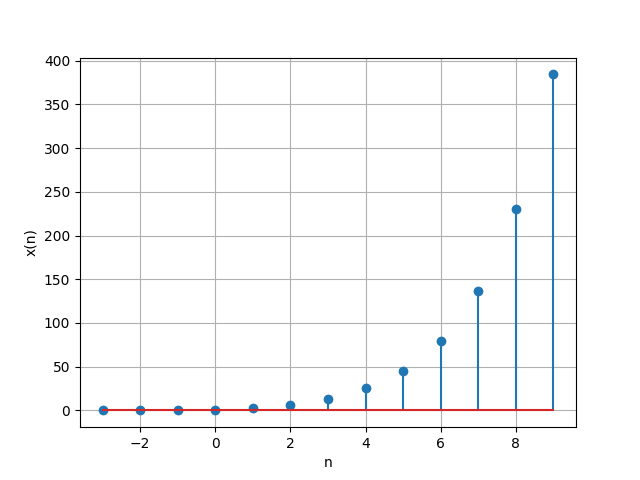
\includegraphics[width = \columnwidth]{2021/EE/31/figs/transform.png}
	\caption{$x(n) vs n $ using $a = 1.5$}
    \label{fig:graph1.41.IN.2022}
\end{figure}


\pagebreak

\item The sum of the infinite geometric series
\begin{align}
    1 + \frac{1}{3} + \frac{1}{3^2} + \frac{1}{3^3} + ... \nonumber
\end{align}
(rounded off to one decimal place) is \_\_\_\_\_.
\hfill(GATE 2021 BT Q20)\\
\solution
\iffalse
\let\negmedspace\undefined
\let\negthickspace\undefined
\documentclass[journal,12pt,twocolumn]{IEEEtran}
\usepackage{cite}
\usepackage{amsmath,amssymb,amsfonts,amsthm}
\usepackage{algorithmic}
\usepackage{graphicx}
\usepackage{textcomp}
\usepackage{xcolor}
\usepackage{txfonts}
\usepackage{listings}
\usepackage{enumitem}
\usepackage{mathtools}
\usepackage{gensymb}
\usepackage{comment}
\usepackage[breaklinks=true]{hyperref}
\usepackage{tkz-euclide} 
\usepackage{listings}
\usepackage{gvv}                            \usepackage{tikz}
\usepackage{circuitikz}
\def\inputGnumericTable{}                                
\usepackage[latin1]{inputenc}                            
\usepackage{color}                                       
\usepackage{array}                                       
\usepackage{longtable}                                   
\usepackage{calc}                              
\usepackage{tikz}
\usepackage{multirow}                                    
\usepackage{hhline}                                      
\usepackage{ifthen}                            
\usepackage{caption}
\usepackage{lscape}
\usepackage{amsmath}
\newtheorem{theorem}{Theorem}[section]
\newtheorem{problem}{Problem}
\newtheorem{proposition}{Proposition}[section]
\newtheorem{lemma}{Lemma}[section]
\newtheorem{corollary}[theorem]{Corollary}
\newtheorem{example}{Example}[section]
\newtheorem{definition}[problem]{Definition}
\newcommand{\BEQA}{\begin{eqnarray}}
\newcommand{\EEQA}{\end{eqnarray}}
\newcommand{\define}{\stackrel{\triangle}{=}}
\theoremstyle{remark}
\newtheorem{rem}{Remark}

\begin{document}

\bibliographystyle{IEEEtran}
\vspace{3cm}

\title{GATE 2021 NM Q24}
\author{EE23BTECH11009 - AROSHISH PRADHAN$^{*}$% <-this % stops a space
}
\maketitle
\newpage
\bigskip
\textbf{Question:} The sum of the infinite geometric series
\begin{align}
    1 + \frac{1}{3} + \frac{1}{3^2} + \frac{1}{3^3} + ... \nonumber
\end{align}
(rounded off to one decimal place) is \_\_\_\_\_.
\hfill(GATE 2021 BT Q20)\\
\solution
\fi
\begin{table}[!h]
    \centering
    \begin{tabular}{|c|c|c|}
    \hline
       \textbf{Symbol}  & \textbf{Value} & \textbf{Description}\\
    \hline
        $x(n)$ &  & $(n+1)^{th}$ term of series\\
    \hline
        $x(0)$ & $1$ & $1^{st}$ term of series\\
    \hline
        $r$ & $\frac{1}{3}$ & Common ratio\\
    \hline
        $y(n)$ & & Sum of $(n+1)$ terms\\
    \hline
     \end{tabular}
    \caption{Given Parameters}
    \label{tab:1_gate.21.bt.20}
\end{table}


General term:
\begin{align}
    x(n) &= x(0)r^nu(n)\\
    \implies X(z) &= \frac{1}{1-rz^{-1}}\\
    y(n) &= x(n) \ast u(n)\\
    \implies Y(z) &= X(z)U(z)\\
    &= \frac{1}{(1-rz^{-1})(1-z^{-1})}\\
    &= \frac{1}{r-1}\brak{\frac{r}{1-rz^{-1}} - \frac{1}{1-z^{-1}}}\\
\end{align}
Taking inverse Z-transform:
\begin{align}
    y(n) &= \frac{1}{r-1}\brak{r(r^nu(n)) - u(n))}\\
    &= \brak{\frac{r^{n+1} - 1}{r - 1}}u(n)\\
    &= \brak{\frac{1 - r^{n+1}}{1 -  r}}u(n)
\end{align}
For infinite terms:
\begin{align}
    y(\infty) &= \lim_{n \rightarrow \infty} \brak{\frac{1 - r^{n+1}}{1 -  r}}u(n)\\
    &= \frac{1}{1-r}\\
    &= \frac{3}{2}
\end{align}

\begin{figure}[!h]
    \centering
    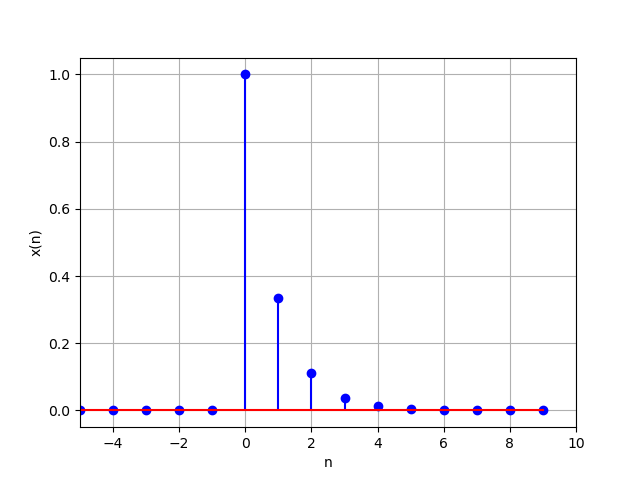
\includegraphics[width = \columnwidth]{2021/BT/20/figs/x_plt.png}
    \caption{Plot of $x(n)$ vs $n$}
    \label{fig:1_gate.21.bt.20}
\end{figure}
\begin{figure}[!h]
    \centering
    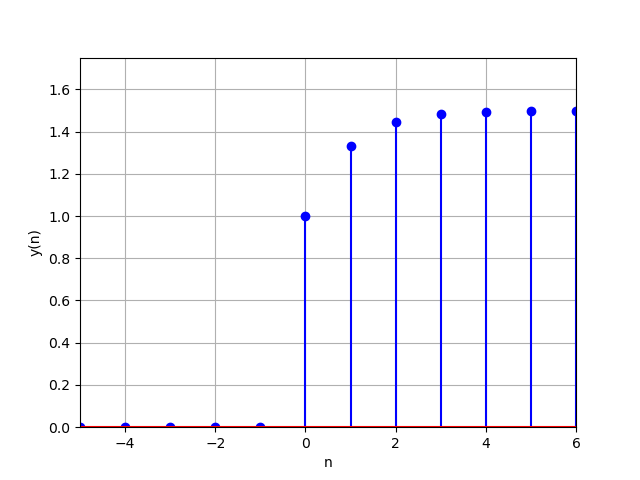
\includegraphics[width = \columnwidth]{2021/BT/20/figs/y_plt.png}
    \caption{Plot of $y(n)$ vs $n$}
    \label{fig:2_gate.21.bt.20}
\end{figure}
%\end{document}


\pagebreak
\item If x is an integer with  x$>$1, the solution of 
\begin{align*}
\lim_{x\to\infty}\left(\frac{1}{x^2}+\frac{2}{x^2}+\frac{3}{x^2}+\cdots+\frac{x-1}{x^2}+\frac{1}{x}\right)
\end{align*}
\begin{enumerate}[label=\alph*)]
\item Zero 
\item 0.5 
\item 1.0 
\item $\infty$  \hfill{\brak{GATE\ 2021\ AG\ Q.2}}
\end{enumerate}
\solution
\iffalse
\let\negmedspace\undefined
\let\negthickspace\undefined
\documentclass[journal,12pt,twocolumn]{IEEEtran}
\usepackage{cite}
\usepackage{amsmath,amssymb,amsfonts,amsthm}
\usepackage{algorithmic}
\usepackage{graphicx}
\usepackage{textcomp}
\usepackage{xcolor}
\usepackage{txfonts}
\usepackage{listings}
\usepackage{enumitem}
\usepackage{mathtools}
\usepackage{gensymb}
\usepackage{comment}
\usepackage[breaklinks=true]{hyperref}
\usepackage{tkz-euclide} 
\usepackage{listings}
\usepackage{gvv}                                        
\def\inputGnumericTable{}                                 
\usepackage[latin1]{inputenc}                                
\usepackage{color}                                            
\usepackage{array}                                            
\usepackage{longtable}                                       
\usepackage{calc}                                             
\usepackage{multirow}                                         
\usepackage{hhline}                                           
\usepackage{ifthen}                                           
\usepackage{lscape}
%\usepackage[export]{adjustbox}

\newtheorem{theorem}{Theorem}[section]
\newtheorem{problem}{Problem}
\newtheorem{proposition}{Proposition}[section]
\newtheorem{lemma}{Lemma}[section]
\newtheorem{corollary}[theorem]{Corollary}
\newtheorem{example}{Example}[section]
\newtheorem{definition}[problem]{Definition}
\newcommand{\BEQA}{\begin{eqnarray}}
\newcommand{\EEQA}{\end{eqnarray}}
\newcommand{\define}{\stackrel{\triangle}{=}}
\theoremstyle{remark}
\newtheorem{rem}{Remark}
\begin{document}
\parindent 0px
\bibliographystyle{IEEEtran}

\title{GATE 2021 AG -Q.2}
\author{EE23BTECH11220 - R.V.S.S Varun$^{}$% <-this % stops a space
}
\maketitle
\newpage
\bigskip

\renewcommand{\thefigure}{\theenumi}
\renewcommand{\thetable}{\theenumi}
\section*{Question}
If x is an integer with  x$>$1, the solution of 
\begin{align*}
\lim_{x\to\infty}\left(\frac{1}{x^2}+\frac{2}{x^2}+\frac{3}{x^2}+\cdots+\frac{x-1}{x^2}+\frac{1}{x}\right)
\end{align*}
\begin{enumerate}[label=\alph*)]
\item Zero 
\item 0.5 
\item 1.0 
\item $\infty$  \hfill{\brak{GATE\ 2021\ AG\ Q.2}}
\end{enumerate}
\fi
\begin{table}[h]
    \centering
      \begin{tabular}{|c|c|c|}
    \hline
    Parameter & Description & Value \\
    \hline
      p\brak{n}   & $\brak{n+1}^{th}$ term of the sequence& $\dfrac{n+1}{x^2}$\\
    \hline
       q\brak{n}  & sum of \brak{n+1} terms of the sequence & - \\
    \hline
    \end{tabular}

 \caption{Table of parameters}
    \label{tab:AG.2.1}
\end{table}

From table ,
\begin{align}
	P\brak{z}=\frac{1}{x^2}\sum_{n=-\infty}^{n=\infty}\brak{n+1}u\brak{n}z^{-n} \label{AG.2.1}
\end{align}
\begin{align}
	n^2 u\brak{n}\xleftrightarrow{\mathcal{Z}} \frac{z^{-1}\brak{z^{-1}+1}}{\brak{1-z^{-1}}^3} ,  \abs{z} > 1 \label{ag.2.1}\\
	n u\brak{n}\xleftrightarrow{\mathcal{Z}} \frac{z^{-1}}{\brak{1-z^{-1}}^2} ,   \abs{z} >1 \label{ag.2.2}\\
   u\brak{n}\xleftrightarrow{\mathcal{Z}} \frac{1}{\brak{1-z^-1}} ,   \abs{z} >1  \label{ag.2.3}
\end{align}
From \eqref{AG.2.1}
\begin{align}
	P\brak{z}&=\frac{1}{x^2}\frac{1}{\brak{1-z^{-1}}^2} , \abs{z} >1\\
	q\brak{n}&=p\brak{n}\ast u\brak{n}\\
	\implies Q\brak{z}&=P\brak{z}U\brak{z}   \\
	&=\brak{\frac{1}{x^2}\frac{1}{({1-z^{-1})}^{2}}}\brak{\frac{1}{1-z^{-1}}}  \\
	 &=\frac{1}{x^2}\frac{1}{({1-z^{-1})}^{3}} ,\quad \abs{z}>1 \label{ag.2.4}
\end{align}

Using $Z$-transform pairs \eqref{ag.2.1} ,\eqref{ag.2.2} ,\eqref{ag.2.3} to find the inverse $Z$-transform,
\begin{align}
	\frac{1}{\brak{1-z^{-1}}^{3}} = \frac{1}{\brak{1-z^{-1}}}+\frac{3z^{-1}}{2\brak{1-z^{-1}}^2}+\frac{z^{-1}\brak{z^{-1}+1}}{2\brak{1-z^{-1}}^3} \label{ag.2.5}
\end{align}
From equations \eqref{ag.2.4} ,\eqref{ag.2.5}
\begin{align}
	q\brak{n}&=\frac{1}{x^2}\brak{\frac{n^2}{2}+\frac{3n}{2}+1} \\
	&=\frac{1}{x^2}\frac{\brak{n+1}\brak{n+2}}{2}
 \end{align}
 put $n=x-1$ to obtain the sum of first x terms
 \begin{align}
	q\brak{x-1}&=\frac{1}{x^2}\frac{\brak{x}\brak{x+1}}{2} 
\end{align}
\begin{align}
    \lim_{x\to\infty}q\brak{x-1}=\frac{1}{2}
\end{align}
Hence , option \brak{B} is correct.


\pagebreak
\end{enumerate}
